%%%%%%%%%%%%%%%%%%%%%%%%%%%%%%%%%%%%%%%%%%%%%%%%%%%%%%%%%%%%%%%%%%%%%%
%
%     This is a LaTex template to be used for a PhD thesis in the
%     Department of Physics at Carnegie Mellon University. It is
%     recommended to input individual chapters, appendices, etc
%     as separate files. To avoid having to provide multiple files
%     with this template, simple examples for such separate files
%     are included with this template.
%                                                       July 2010
%
%     For comments contact: Manfred Paulini <paulini@cmu.edu>
%
%%%%%%%%%%%%%%%%%%%%%%%%%%%%%%%%%%%%%%%%%%%%%%%%%%%%%%%%%%%%%%%%%%%%%%
%
\documentclass[12pt,twoside,bibliography=totoc]{report}
%
% ====================================================================
%    Packages
% ====================================================================
%
\usepackage{color}
\usepackage{graphicx}
\usepackage{amsfonts,amssymb,amsmath,latexsym,amsthm}
\usepackage{algorithmic}
\usepackage{array}
\usepackage{mdwmath}
\usepackage{mdwtab}
\usepackage{eqparbox}
\usepackage{caption}
\usepackage{subcaption}
\usepackage{stfloats}
\usepackage{url}
\usepackage[space]{cite}
\usepackage{enumitem}
\usepackage{color}
\usepackage{pdfsync}
\usepackage{wrapfig}
\usepackage{import}
\usepackage{multicol}
\usepackage{multirow}
\usepackage{booktabs}
\usepackage{hhline}
\usepackage{epsfig}
\usepackage{setspace}
\usepackage{fancybox}
\usepackage{hyperref}
\hypersetup{
  colorlinks,
  citecolor=black,
  filecolor=black,
  linkcolor=black,
  urlcolor=black
}

\DeclareGraphicsExtensions{.pdf,.jpeg,.png,.eps}
\graphicspath{{figures/}}
\bibliographystyle{plain}

%
% ====================================================================
%    Formatting
% ====================================================================
%
%
% ====================================================================
%    Margins
% ====================================================================
%
\topmargin -0.3in
\oddsidemargin 0.5in
\evensidemargin 0.5in
\textheight 8.5in
\textwidth 6.0in
%
% ====================================================================
%     The following commands tent to keep LaTex happier in the
%     placement of figures, tables, etc
% ====================================================================
%
\renewcommand{\textfraction}{0.0}
\renewcommand{\floatpagefraction}{0.0}
\renewcommand{\topfraction}{1.0}
\renewcommand{\bottomfraction}{1.0}
\setcounter{topnumber}{9}
\setcounter{bottomnumber}{9}
\setcounter{totalnumber}{9}


%
% ====================================================================
%    Author, title, date
% ====================================================================
%
\author{
  \\
        Erik Arthur Nelson \\
        \today \\
  \\
        
\includegraphics[width=0.3\textwidth]{cmu_seal.pdf}
  \\
  \\
        The Robotics Institute \\
        School of Computer Science \\
        Carnegie Mellon University \\
        Pittsburgh, Pennsylvania \\
  \\
        {\bf Thesis Committee:} \\
        Nathan Michael, {\it Chair} \\
        Two \\
        Three \\
  \\
        \textit{Submitted in partial fulfillment of the requirements} \\
        \textit{for the degree of Master of Science in Robotics.}
}

\title{\bf{
  Title Goes Here
}}

% Supress the date
\date{}

%
% ====================================================================
%    Definitions
% ====================================================================
%
\newcolumntype{L}{>{\centering\arraybackslash}m{1.65cm}}
\newtheorem{thm}{Theorem}
\newtheorem{lem}[thm]{Lemma}

\newcommand{\comment}[1]{{\color{magenta}{#1}}}
\newcommand{\todo}[1]{{\color{blue}{#1}}}
\newcommand{\changed}[1]{{\color{red}{#1}}}
\newcommand{\squeeze}[1]{{\vspace{-0.1cm}}}
\newcommand{\remove}[1]{}

%
% ====================================================================
%   Notation
% ====================================================================
%
% Math definitions
\newcommand{\norm}[1]{\left\Vert#1\right\Vert}
\newcommand{\abs}[1]{\left\vert#1\right\vert}
\newcommand{\set}[1]{\left\{#1\right\}}
\newcommand{\To}{\longrightarrow}
\newcommand{\Ker}{\textup{Ker}}
\newcommand{\Img}{\textup{Img}}
\newcommand{\diag}{\textup{diag}}
\newcommand{\circulant}{\textup{circ}}
\newcommand{\bcf}{\;\mbox{\boldmath ${\cal F}$\unboldmath}}
\def\Vec#1{\!\!\hbox{$#1$\kern-0.38em\lower0.85em\hbox{$\vec{}\,$}}\,}%
\newcommand{\bbm}{\begin{bmatrix}}
\newcommand{\ebm}{\end{bmatrix}}
\newcommand{\mbf}[1]{\mathbf{#1}}
\newcommand{\mbs}[1]{{\boldsymbol{#1}}}
\newcommand{\mbb}[1]{{\mathbb{#1}}}
\newcommand{\mc}[1]{\mathcal{#1}}
\newcommand{\argmin}{\operatornamewithlimits{argmin}}
\newcommand{\argmax}{\operatornamewithlimits{argmax}}
\newcommand{\expect}{\operatornamewithlimits{\mbb{E}}}
\newcommand{\eq}[1]{\begin{align}\begin{split}#1\end{split}\end{align}}
\newcommand*{\bigcdot}{\raisebox{-0.25ex}{\scalebox{1.2}{$\cdot$}}}

%

\begin{document}
\thispagestyle{empty}
\maketitle

% ====================================================================
%     Single blank page before the abstract
% ====================================================================
%
%\thispagestyle{empty} \cleardoublepage
%

% ====================================================================
%    Abstract
% ====================================================================
%
\doublespacing
\begin{abstract}
\end{abstract}

\singlespacing
%

% ====================================================================
%     Single blank page after the abstract
% ====================================================================
%
\thispagestyle{empty} \cleardoublepage
\pagenumbering{roman}
%

% ====================================================================
%    Acknowledgements
% ====================================================================
%
\doublespacing
\section*{Acknowledgements}

I have had the great fortune of working alongside many incredibly talented people
during my time in the Robotics Institute, all of whom contributed in some part to
this thesis and to my future. I am thankful to those who have given me support
and encouragement through what most consider to be a selfish endeavor.

I would first like to thank Prof. Nathan Michael, my advisor, for his immense
help in shaping my research interests, providing critical writing and
presentation feedback, and for the significant one-on-one time that he put into teaching me
the art and science of robotics. Nate, you are the hardest working person that I know,
and it is reflected in the great things that you accomplish.

The members of the Robust Adaptive Systems Lab (RASL) have been an invaluable
resource for solving difficult problems, and for providing hope and comfort
during stressful times. I am thankful to Vishnu Desaraju, John Yao,
Derek Mitchell, and Shihyun Lo for putting everything into perspective, and for
guidance through tricky problems in planning, state estimation, and control
theory.

My experiences at Carnegie Mellon University would not have been nearly as
enjoyable or productive without the friends that I made along the way. Thank you
Nick Gisolfi, Zach Batts, and Allie Del Giorno for balancing my life with music,
philosophy, politics, exercise, and... more robotics.

Finally, I would like to thank the people in my life that guided me into doing
what I now love. Thanks to Profs. Zo\"{e} Wood, Jane Lehr, and Chris Clark, who
encouraged and persuaded me to attend graduate school in the first place.
Thanks to Alex Viksne, my parents, and my sister, who supported me unconditionally.

\singlespacing
%

% ====================================================================
%     Table of contents, list of figures/tables
% ====================================================================
%
%\onehalfspacing
\doublespacing
\tableofcontents
\listoftables
\listoffigures
\clearpage
\pagenumbering{arabic}
%

% ====================================================================
%    Chapter 1
% ====================================================================
%
\chapter{Introduction}
\label{chapter1}

Robots are emerging from controlled factories and
laboratories into our homes, workplaces, roads, and public airspaces.
Alongside their transition into these unstructured and transient environments
comes their need to be able to explore, characterize, and catalog their surroundings.
Mobile robot autonomy is generally accomplished by referring to a map - a 2D or 3D
probabilistic representation of the locations of obstacles in the robot's workspace.
With access to a map, robots can localize to determine their position, plan collision-free
trajectories to goals, locate objects for interaction, and make decisions by
reasoning about the geometry and dynamics of the world. Given that a robot's map
is of critical importance for most autonomy tasks, robots that find
themselves initialized without a priori access to a map should be capable of
autonomously, efficiently, and intelligently creating one.

The exercise of choosing and executing actions that lead a robot to learn more about its own
map is known as \textit{active perception} or \textit{exploration}, and
is the central topic of this thesis. Active perception has previously been studied with a
multitude of sensor models, environment representations, and robot dynamics
models. The active perception task itself can be dissected into two
components~\cite{shen20113d}:

\begin{enumerate}[leftmargin=3.2cm]
  \item[\bf component 1:] Identifying regions in the environment that, when visited, will
    spatially extend or reduce uncertainty in the current map
  \item[\bf component 2:] Autonomously navigating to the aforementioned regions, while
    simultaneously localizing to the map and updating it with acquired sensor
    measurements
\end{enumerate}

A motivating example is depicted in Fig.~\ref{fig:motivation}, where a household
service robot is initialized in an unknown environment. Prior to accomplishing
tasks that a human might ask it to perform, the robot must learn its
surroundings and build a map of the house. Ideally this phase of
initialization would be fast, as it is a prerequisite to the main functionality
of the robot, and also might be required when furniture is moved or
household objects are displaced. Where should the robot travel to observe the
most of the environment in the shortest amount of time? Virtually any autonomous robot
operating in an unknown environment will require a map-building
initialization phase, welcoming strategies that enable high-speed and intelligent
exploration.

\begin{figure}[t]
  \centering
  
\includegraphics[width=0.6\textwidth]{example-image.png}
  \caption{A household service robot awakes in an unknown environment. Prior to
  accomplishing its main functionalities, it will require a map of its surroundings.
What sequence of actions should it take to minimize the time it spends
exploring? \label{fig:motivation}}
\end{figure}

This thesis introduces an assortment of information-theoretic optimizations that
increase the efficiency of active perception when using a beam-based sensor
model (e.g. LIDAR, time-of-flight cameras, structured light sensors) and
an occupancy grid map~\cite{elfes1989using}. Applying these optimizations during exploration allows a
robot to consider a significantly larger number of future locations to move
towards in its partially observed environment, regardless of the planning
strategy used. Additionally, this thesis presents a method for analyzing the
complexity of the local environment and adapting the robot's map resolution,
planning frequency, movement speed, and exploration behaviors accordingly. By
adapting these properties online, an autonomously exploring robot is able to speed up
through areas with open expanses or where the map is well-known, and slow down
when the local environment requires careful maneuvering or more thorough
investigation.

\section{Previous Work}

Prior approaches to mobile robot active perception fall into two
broad categories: \textit{geometric} approaches that reason about the locations and
presence of obstacles and free space in the robot's
map~\cite{acar2002sensor,chan1993line,wang2007view,
burgard2000collaborative,taylor1993exploration,yamauchi1997frontier}, and more
recently, \textit{information-theoretic} approaches that treat the map as
a multivariate random variable and choose actions that will maximally reduce its
uncertainty~\cite{amigoni2010information,bourgault2002information,charrow2015icra,
julian2013mutual,feder1999adaptive}. Both categories of approaches solve {\bf
component 1} of active perception, and assume that a planner and Simultaneous
Localization and Mapping (SLAM) framework are available to accomplish {\bf
component 2}.

\subsection{Geometric Exploration Strategies}

Many successful geometric exploration approaches build upon the seminal work of
Yamauchi~\cite{yamauchi1997frontier}, guiding the robot to \textit{frontiers} - regions on the boundary
between free and unexplored space in the map (Fig.~\ref{fig:frontiers}).
Since multiple frontiers often exist simultaneously in a partially explored map, a
variety of heuristics and spatial metrics can be used to decide which frontier to
travel towards~\cite{lavalle2006planning}. For example, an agent may decide to
visit the frontier whose path through the configuration space from the agent's current
position has minimum length, or requires minimal time or energy input to
traverse. Similarly, an agent may decide to only plan paths to locations
from which frontiers can be observed by its onboard sensors.

\begin{figure}[t]
  \centering
  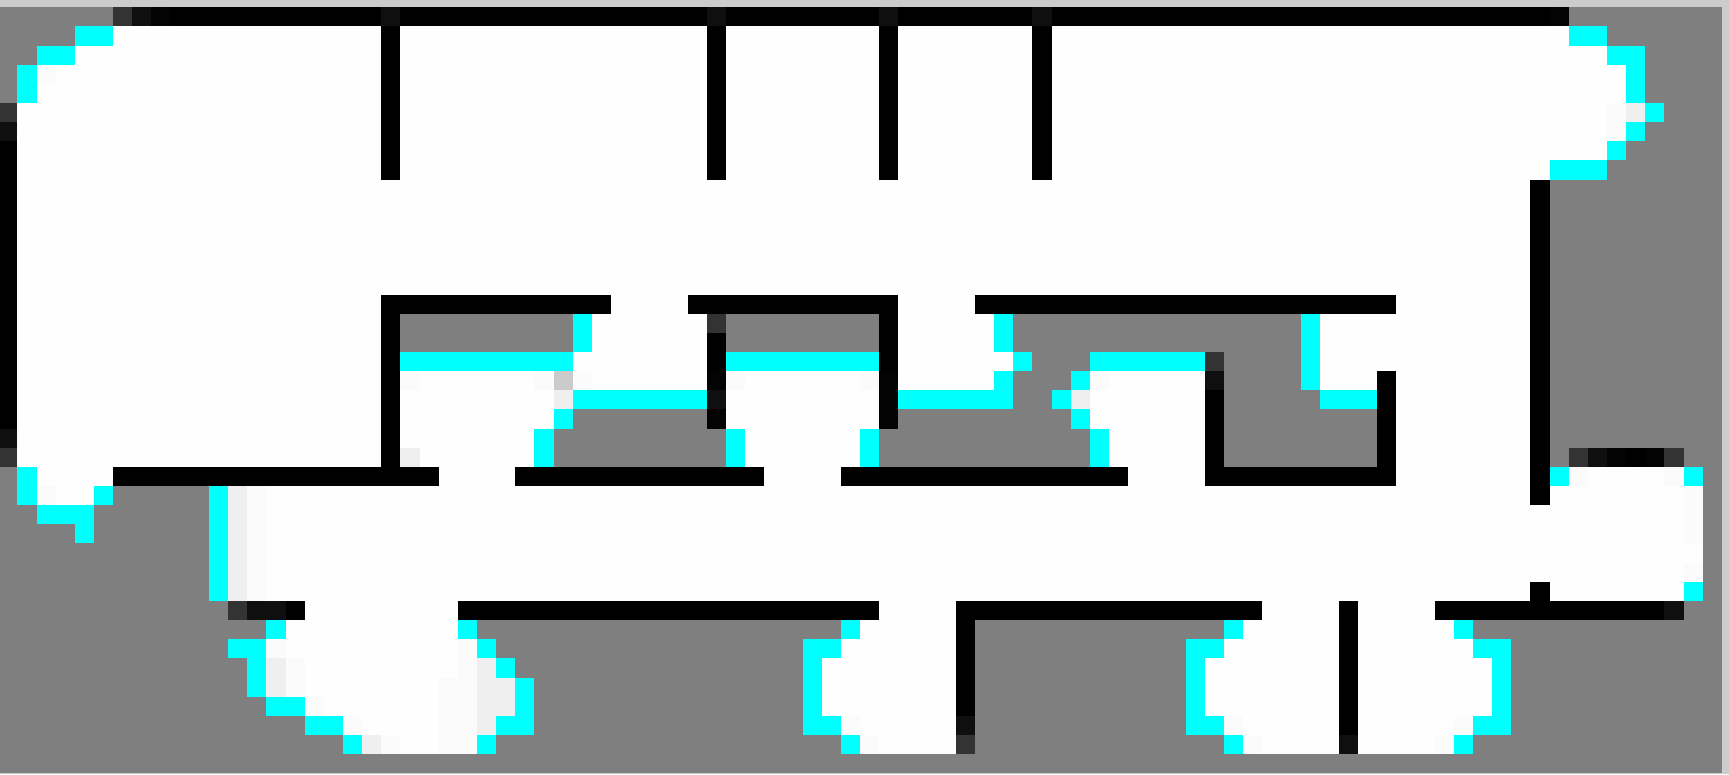
\includegraphics[trim=0cm 0.4cm 0.1cm 0.1cm, clip, width=0.8\textwidth]{frontiers.pdf}
  \caption{A partially explored map with frontiers between free and unknown
  space highlighted in blue.\label{fig:frontiers}}
\end{figure}

While effective in 2D environments, frontier exploration algorithms have
several restrictive qualities. First, the na\"{i}ve extension of frontier exploration
from 2D to 3D maps poses a non-trivial challenge; as the
dimensionality of the workspace increases, frontiers are distributed more
densely throughout the environment due to occlusions, sensing resolution, and
field-of-view, resulting in poor exploration performance~\cite{shen20113d}.
Second, planning a path to a frontier does not imply that the path
itself will be information-rich. Trajectory optimization techniques that
consider information acquired by the robot's sensors along a planned path can be used
as extensions to improve exploration performance~\cite{sim2004online,kollar2008trajectory}.
Finally, although the robot is guaranteed to learn new information upon reaching a
frontier, the amount of information learned is dependent on the
robot's sensor model, which is not considered when identifying frontiers.
It may therefore be more efficient to visit a frontier that is
suboptimal according to heuristics such as path length if the robot's sensors
will provide more information from that location
(Fig.~\ref{fig:sensor_frontier}).
This limitation was first overcome by evaluating the informativeness of simulated
sensor measurements taken from frontier locations~\cite{gonzalez2002navigation}, and was the
original motivation for developing a category of information-theoretic exploration strategies.

\begin{figure}[t]
  \centering
  \centering
  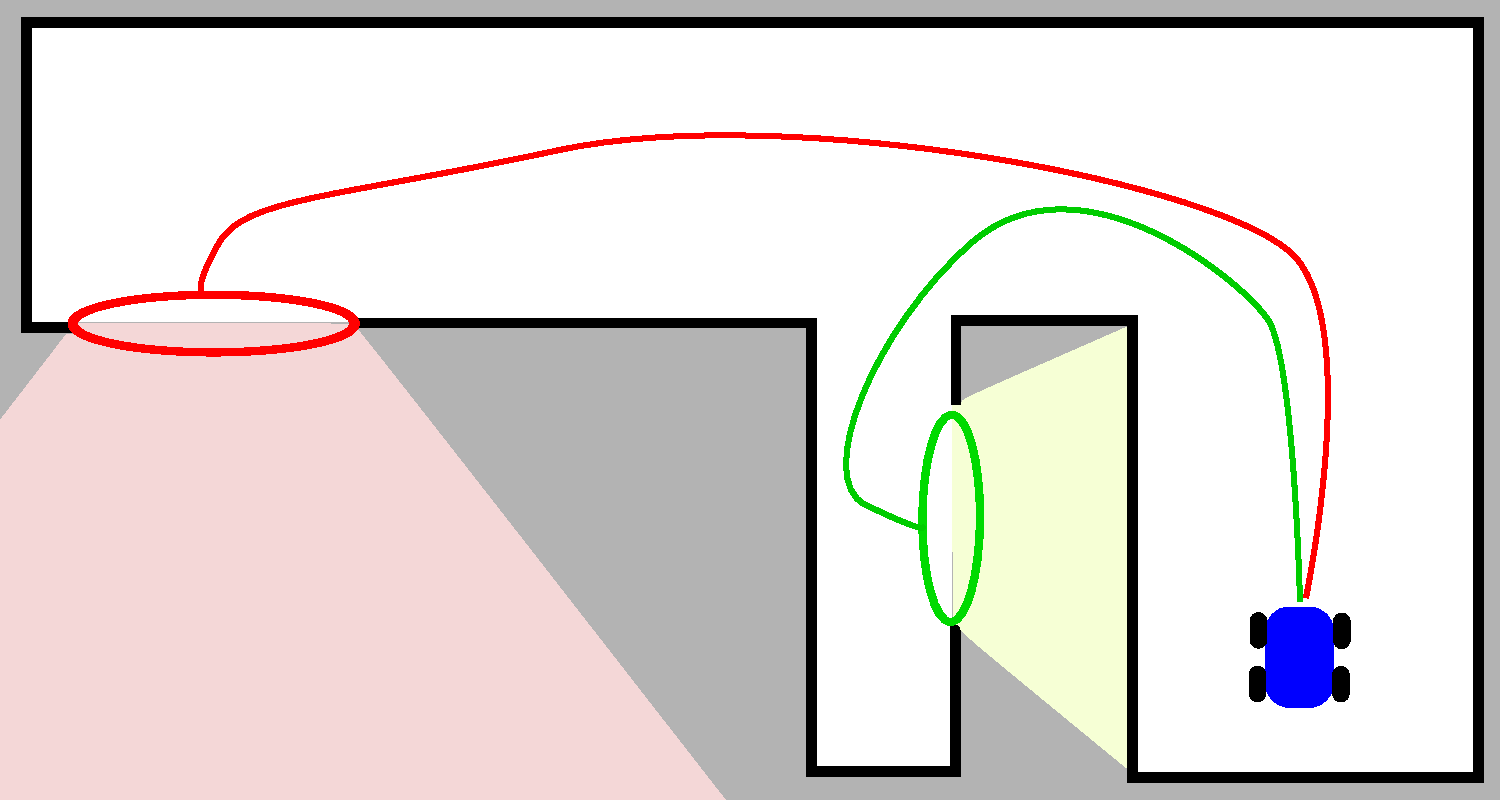
\includegraphics[width=0.7\textwidth]{sensor_frontier.pdf}
  \caption{Traditional frontier exploration would visit the green location first
    because it is closest. A simple extension involves simulating sensor
    measurements from frontiers and examining their informativeness~\cite{gonzalez2002navigation}. Applying this
    extension would cause robot to visit the red frontier first, since that
    location will provide more information about the map per unit time.\label{fig:sensor_frontier}}
\end{figure}

More thorough surveys of frontier exploration algorithms and heuristics are provided by
Basilico et al.~\cite{basilico2008evaluating} and Holz et al.~\cite{holz2011comparative}.

\subsection{Information-Theoretic Exploration Strategies}

Information-theoretic exploration strategies cast the active perception task as
an optimization, and choose actions for the robot that maximize an information-based objective function such
as Shannon's entropy or mutual
information~\cite{bourgault2002information,kollar2008efficient,charrow2015icra,julian2013mutual}
(Fig.~\ref{fig:mi_vs_csqmi}).
Entropic measures like these are appealing because unlike geometric methods,
they capture the relationship between sensor placement and uncertainty in the
map. In addition, they can be computed without a maximum likelihood map estimate, and
therefore do not discard probabilistic information known to the robot. Control policies
that maximize mutual information have been proven to guide robots
towards unexplored space~\cite{julian2013mutual}, and weighting frontiers by
the expected mutual information between the map and a sensor measurement
acquired at the frontier location has been shown to result in more efficient exploration
behaviors than traditional frontier exploration~\cite{charrow2015icra}.
The exact same calculation can be used to evaluate information-theoretic objective
functions in 2D and 3D environments.

\begin{figure}[t]
    \centering
    \begin{subfigure}[t]{0.31\textwidth}
        \centering
        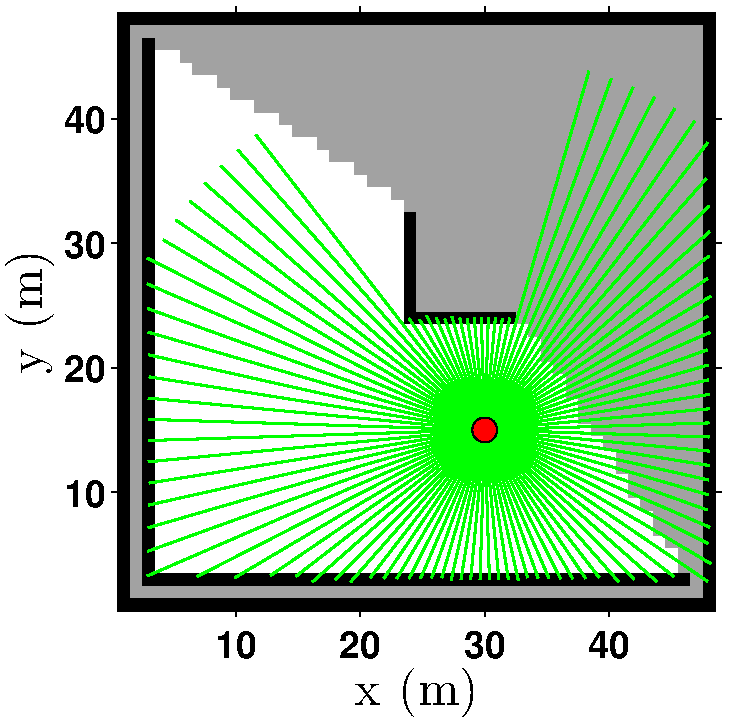
\includegraphics[height=4.0cm]{map.pdf}
        \caption{\label{fig:og}}
    \end{subfigure}
    \begin{subfigure}[t]{0.31\textwidth}
        \centering
        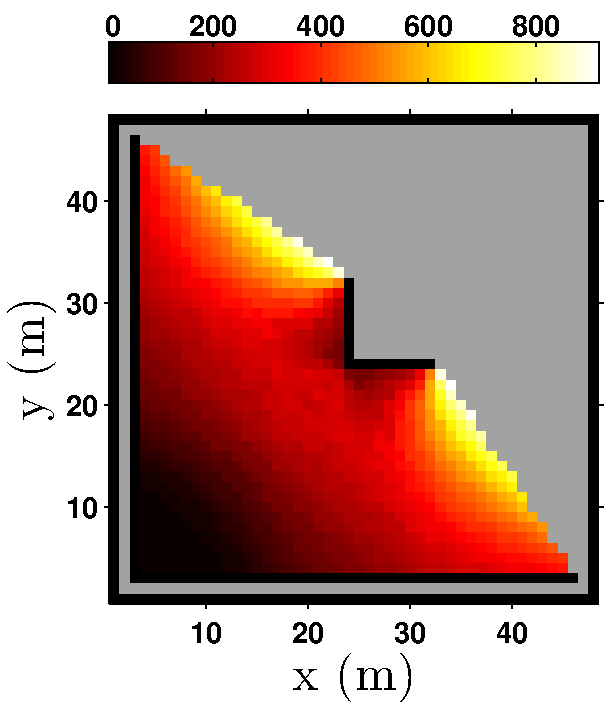
\includegraphics[height=5.0cm]{mi_map.pdf}
        \caption{\label{fig:og_mi}}
    \end{subfigure}
    \begin{subfigure}[t]{0.31\textwidth}
        \centering
        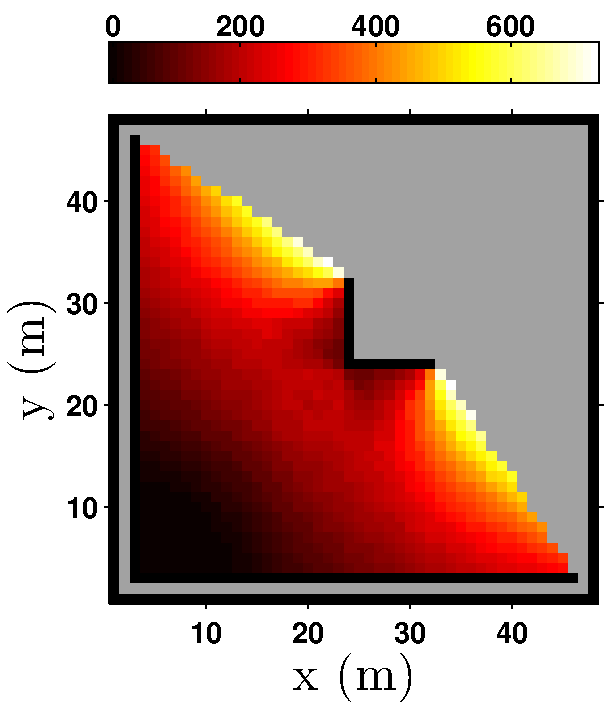
\includegraphics[height=5.0cm]{csqmi_map.pdf}
        \caption{\label{fig:og_csqmi}}
    \end{subfigure}
    \caption{Two variants of mutual information (Fig.~\ref{fig:og_mi}: Shannon;
    Fig.~\ref{fig:og_csqmi}: Cauchy-Schwarz Quadratic) densely computed in free space
  over an occupancy grid (Fig.~\ref{fig:og}) using a $100$-beam omnidirectional 2D
laser with $30$ m range. An exemplary sensor measurement is depicted in
Fig.~\ref{fig:og}. Controlling the robot towards locations that maximize either variant
of mutual information would attract the robot to locations from which it
could observe unknown areas of the map. \label{fig:mi_vs_csqmi}}
\end{figure}

The utility afforded by information-theoretic approaches comes at the cost of
computational inefficiency.
As a point of comparison, frontiers and other geometrically-defined landmarks
need only to be computed once per map update, and can be computed (at worst, using a brute force search)
with time complexity linear in the number of cells in the robot's map.
One may alternatively choose to identify and cache frontiers every time a sensor
measurement is used to update the map, yielding a constant time frontier
identification step that is bounded by the number of map voxels within the maximum sensor range.
By contrast, information-theoretic objective functions typically consider the probabilistic
uncertainty associated with the sensor and environment models, and therefore
require expensive sensor-related operations such as raycasts or sampling a large
number of times from the distribution of possible future measurements.
Approximations to mutual information between a map and beam-based sensor
measurements can be evaluated with time complexity linear in the number of map
voxels intersected by a sensor's
beams~\cite{julian2013mutualthesis,charrow2015icra,nelson2015iros}. This
already-expensive operation must be performed for every future location that the
robot might wish to travel to. Julian et al. report that densely calculating
mutual information over the free space in a large $1500$ m$^{2}$ map requires
approximately ten seconds with a parallelized implementation using a $3.4$ Ghz
quad-core CPU and NVIDIA GTX 690 graphics card~\cite{julian2013mutual}.

\section{Thesis Problem}

Although inefficient, information-theoretic solutions to the active perception task
are superior to geometric solutions in many ways. However, modern computers cannot densely
evaluate information-theoretic objective functions over a robot's map in real-time.
Any strategy that makes the evaluation of information-theoretic objective functions more
efficient will allow a robot to consider more future locations prior to taking
an action towards one, thereby increasing the speed at which the robot is able
to explore an environment.

Currently, the most efficient information-theoretic exploration algorithms are
too slow for the motivating scenario described in
Fig.~\ref{fig:motivation}. For example, a highly-efficient recent approach
by Charrow et al., requires eleven minutes to explore a $17$ m $\times 18$ m $
\times 3$ m building with a quadrotor - enough time for the quadrotor's batteries to
deplete twice~\cite{charrow2015icra}. This thesis addresses the inefficiencies of information-theoretic exploration,
summarized in the following statement:

% Thesis Problem
\begin{center} \fbox{
  \parbox{0.9\linewidth}
  { {\bf Thesis Problem:} Solutions to the mobile robot active perception task
  that involve optimization of information-theoretic cost functions are too
  computationally expensive for high-speed exploration in complex environments.}
} \end{center}

\section{Thesis Statement}

This thesis proposes occupancy grid compression as a solution to
the computational inefficiencies of information-theoretic exploration.

\section{Outline}





%

% ====================================================================
%    Chapter 2
% ====================================================================
%
\chapter{Active Perception Foundations}
\label{chapter2}

This thesis draws upon prior research from the robotics, information theory, and signal
processing domains to develop its formulations.
Sections~\ref{sec:occ_grid_mapping} - \ref{sec:action_generation} review relevant topics within
robotics including occupancy grid mapping,
active perception as an optimization, and several planning strategies that are suitable for the
exploration task. These foundational topics will be used to develop a theory of
optimal occupancy grid compression as well as methods for guiding a robot to explore
uncertain areas of its map efficiently. The formulations developed in
Chapters~\ref{chapter3} - \ref{chapter5} will also
borrow heavily from information theory and rate distortion theory. These
domains are frequently concerned with evaluating the effect one random
variable (e.g. a sensor measurement) has on
another (e.g. a map) or with compressing a random variable to a reduced
representation in such a way that the compressed form preserves the structure of the
uncompressed form.
Sections~\ref{sec:entropy_and_divergence} and \ref{sec:csqmi} review concepts from
these domains that will be used when developing theories for optimal map resolution selection,
for adapting robot exploration behaviors to the map's resolution, and for
selecting informative trajectories that drive through obstacle-free areas of the map.

\section{Occupancy Grid Mapping}
\label{sec:occ_grid_mapping}

Occupancy grids (OGs) are a common and useful proabilistic map model for representing and
reasoning about an unknown environment~\cite{elfes1989using}. The remainder of this thesis assumes that the robot's environment is represented as an OG.  Figures~\ref{fig:motivation},~\ref{fig:frontiers},~\ref{fig:sensor_frontier} and~\ref{fig:og} depict occupancy grids,
where black cells represent areas of the environment occupied by an obstacle, white cells
represent areas that do not contain obstacles, and grey cells represent
locations with unknown occupancy status.

OGs decompose the robot's workspace into a discrete set of 2D or 3D cells with a
specified resolution. The presence or absence of obstacles within these cells is modeled
as a $K$-tuple binary random variable, $\mbf{m} = \{m_{i}\}_{i=1}^{K}$, with support set
$\{\texttt{EMP}, \texttt{OCC}\}$. The probability that an individual cell is occupied is
given by $p\left(m_{i} \ \vert \ \mbf{x}_{1:t}, \mbf{z}_{1:t}\right)$, where $\mbf{x}_{1:t}$ denotes the
robot's history of states, and $\mbf{z}_{1:t}$ denotes the history of range observations
accumulated by the robot. The OG representation treats cells as independent from one another,
allowing one to express the joint occupancy probability of a specific map as the product of individual
cell occupancy probabilities:
%
\eq{
  p\left(\mbf{m} \ \vert \ \mbf{x}_{1:t}, \mbf{z}_{1:t}\right)
  &=
  \prod_{i} p\left(m_{i} \ \vert \ \mbf{x}_{1:t}, \mbf{z}_{1:t}\right).
  \label{eq:og_independence}
}
%
For notational simplicity, the map conditioned on random variables
$\mbf{x}_{1:t}$ and $\mbf{z}_{1:t}$ will henceforth be written as $p\left(\mbf{m}\right)
\equiv p\left(\mbf{m} \ \vert \ \mbf{x}_{1:t}, \mbf{z}_{1:t}\right)$, and the probability of occupancy
for a grid cell $m_i$ as $o_{i}\equiv p\left(m_{i}=\texttt{OCC}\ \vert \
\mbf{x}_{1:t}, \mbf{z}_{1:t}\right)$.
Unobserved grid cells are assigned a uniform prior such that
$\{o_{i} = 1 - o_{i} = 0.5\}_{i=1}^{K}$. This implies that the robot is
initially unaware of its surroundings prior to accumulating sensor measurements.
To prevent numerical precision issues, the
occupancy status of a grid cell $m_i$ is represented by the log-odds ratio
%
\eq{
  l_{i}
  &\equiv
  \log
  \frac{o_{i}}
  {1 - o_{i}}.
}
%
The log-odds ratio maps from occupancy probabilities existing on $[0, 1]$ to
$\mbb{R}$, which is more suitable for floating-point arithmetic. In addition,
the log-odds ratio makes updates to a cell occupancy probability additive rather
than multaplicative. When a new measurement $\mbf{z}_t$ is obtained, a cell's
log-odds  occupancy probability
may be updated with
%
\eq{
  l_{i} &\gets
  l_{i}
  +
  L\left(m_{i}\, \vert \mbf{z}_{t}\right),
}
%
where the term $L\left(m_{i}\,  \vert \mbf{z}_{t}\right)$ represents the robot's inverse sensor model~\cite{thrun2005probabilistic}.

\section{Active Perception as an Optimization}
\label{sec:active_perception}

Active perception is the idea that a machine should continually guide itself to states in
which it is able to acquire better sensor measurements~\cite{bajcsy1988active,bajcsy1992active}.
Active perception draws inspiration from biological sensors that adapt in
response to external stimuli. The human eye, for example, has muscles that
constrict the pupil in response to bright light (adaptation), and others that distort the
curvature of its lens to focus on nearby or far-away objects (accomodation).
Adaptation and accomodation allow humans to see light varying nine orders of
magnitude in brightness, and focus on objects an infinite distance away.
Similarly, a man-made sensor such as a camera should not passively collect and report incoming photons,
but should adapt its aperture, CMOS gains, and shutter speed based on the
properties of the incoming light.

To extend this idea to mobile robotics, one must consider the robot system itself as
a sensor that is able to move and actuate for the purpose of collecting better
sensor measurements. From this perspective, the robot's task is to choose and
execute \textit{actions} that optimize the quality of its sensor measurements.
An action can be defined as a sequence of configurations
$\mbf{x}_{\mbf{\tau}}\equiv \left(\mbf{x}_{t+1}, \dots, \mbf{x}_{t+T}\right)$
that the robot will achieve
over a future time interval $\mbf{\tau}\equiv (t+1,\dots,t+T)$. From configurations
$\mbf{x}_{\mbf{\tau}}$ the robot will acquire future sensor measurements
$\mbf{z}_{\mbf{\tau}} \equiv
\left(\mbf{z}_{t+1}(\mbf{x}_{t+1}), \dots, \mbf{z}_{t+T}(\mbf{x}_{t+T})\right)$. This thesis is
concerned primarily with ground robots constrained to $SE(2)$, and will
therefore use $\mbf{x}_{i}$ to refer to a pose in 2D space: $\mbf{x}_{i}\equiv
\left(x_{i}, y_{i}, \theta_{i}\right)^{T}$.

In the context of exploring an unknown environment, the active perception problem can
be framed as an optimization over possible future actions that the robot can take:
%
\eq
{
  \mbf{x}_{\mbf{\tau}}^{*}
  &=
  \argmax_{\mbf{x}_{\mbf{\tau}} \in \mc{X}}
  \ \mc{J}\left(\mbf{m}, \mbf{z}_{\mbf{\tau}}(\mbf{x}_{\mbf{\tau}})\right),
  \label{eq:active_perception}
}
%
where $\mc{J}\left(\mbf{m}, \mbf{z}_{\mbf{\tau}}(\mbf{x}_{\mbf{\tau}})\right)$ is a reward
function expressing the new information learned by sequentially moving the robot
to configurations $\mbf{x}_{\mbf{\tau}}$, collecting sensor measurements
$\mbf{z}_{\mbf{\tau}}$, and updating the map $\mbf{m}$. $\mc{X}$ is the set of all collision-free
and dynamically feasible actions that the robot can take. In addition to
evaluating the pure information content of $\mbf{z}_{\mbf{\tau}}$, $\mc{J}$ commonly
incorporates the time or energy expenditure required to carry out the
action $\mbf{x}_{\mbf{\tau}}$.

Unfortunately, the active perception optimizaton faces the \textit{curse of dimensionality};
the size of $\mc{X}$ grows exponentially with the length of the time horizon $\tau$.
As $\tau$ increases in size, it quickly becomes infeasible to evaluate $\mc{J}$ over all
possible actions in $\mc{X}$. This inefficiency is the primary reason that dense
evaluation of a reward function over a map is infeasible for high planning
frequencies. Instead, to remain computationally tractable, one can generate a
fixed-size set of candidate actions that are likely to be informative prior to
optimizing~\eqref{eq:active_perception}. Because the candidate action set is a
subset of $\mc{X}$, it is possible, and in many situations likely, that the most
informative possible action will not be considered.

\section{Action Generation}
\label{sec:action_generation}

The primary concern of action generation is to suggest a fixed-size set of feasible actions
$\hat{\mc{X}}$ that are likely to be informative. A suitable choice of $\mc{J}$ can be
evaluated on these actions to choose an optimal exploration action
using~\eqref{eq:active_perception}. Several
action generation options exist.

\subsection{Frontier Seeding}
\label{subsec:frontier_seeding}

Recent works by Charrow et al.~\cite{charrow2015icra} and Vallv\'{e} et
al.~\cite{vallve2014dense} suggest seeding
information-theoretic exploration by identifying frontiers and then evaluating
a reward function from frontier locations. Because frontier
identification is efficient, this two-pass approach is useful for locating
potentially informative locations prior to performing the comparatively more
expensive reward evaluation step. This strategy has the added benefit that frontiers are computed
globally across the robot's map, guaranteeing that the robot will never become
trapped in a dead-end or a location where its local map is already fully
explored (i.e. a local minimum in information space).

Identifying frontiers before planning to them avoids planning
trajectories to many future locations in a single planning cycle. Frontiers can be ranked by the
information-theoretic reward offered from their locations, and the resulting sorted list
of frontiers can be iterated through until a dynamically feasible and
collision-free trajectory is found. Planning from an initial state to a goal state
subject to dynamic and obstacle constraints becomes especially expensive in
high-dimensional configuration spaces, and should be performed as few times as possible.

After selecting a location that will yield high reward,
one may use a real-time pathfinding algorithm such as A*~\cite{hart1968formal},
RRT~\cite{lavalle1998rapidly}, or their many variants to generate a trajectory from
the robot's initial state.

\subsection{Forward-Arc Motion Primitives}
\label{subsec:fa_motion_primitives}

Actions can also be generated by sampling from a set of
pre-computed motion primitives. A simple strategy for generating motion
primitives for a ground vehicle constrained to $SE(2)$ involves
simulating the robot's path when moving at a constant linear and angular
velocity for a specified amount of time.
Actions resulting from this approach form arcs of a circle with a radius that is a
function of the specified linear and angular velocity (Fig.~\ref{fig:motion_prims}).

Consider a robot following the arc of a
circle with velocity $v$ and rotational velocity $\omega$. Assuming the robot's
current position is given by $\mbf{x}_t=(x_t,y_t,\theta_t)^T$, forward-arc motion primitives
can be generated by specifying the future robot state, $\mbf{x}_{t+T}$,
as a function of $v$ and $\omega$ for a sequence of uniformly varying
times $T \in \mbb{R}^{+}$. These paths are described
by a set of nonlinear differential equations:
%
\eq{
  \dot{\mbf{x}}_{t+T}
  &=
  \bbm
  \dot{x} \\
  \dot{y} \\
  \dot{\theta}
  \ebm_{t+T}
  =
  \bbm
  v \cos
  \left(
  \theta_{t+T}
  \right) \\
  v \sin
  \left(
  \theta_{t+T}
  \right) \\
  \omega
  \ebm,
  \label{eq:arc_differential}
}
%
the solution of which is given by
%
\eq{
  \mbf{x}_{t+T}
  &=
  \bbm
  \frac{v}{\omega}
  \left(
  \sin
  \left(
  \omega T + \theta_{t}
  \right)
  -
  \sin
  \left(
  \theta_{t}
  \right)
  \right)
  \\
  \frac{v}{\omega}
  \left(
  \cos
  \left(
  \theta_{t}
  \right)
  -\cos
  \left(
  \omega T + \theta_{t}
  \right)
  \right)
  \\
  \omega T
  \ebm
  +
  \mbf{x}_{t}.
  \label{eq:motion_primitive_generator}
}
%
Sequentially incrementing $T$ in~\eqref{eq:motion_primitive_generator}
produces a sampling of poses lying along an arc
parameterized by the robot's velocity and angular velocity, with origin $\mbf{x}_{t}$.

\begin{figure}[t]
  \centering
  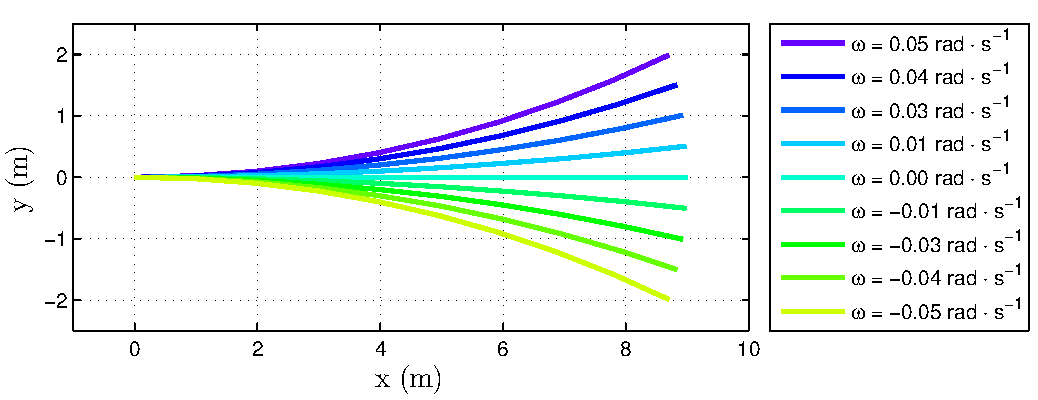
\includegraphics[width=0.9\textwidth]{motion_primitives.pdf}
  \caption[A forward-arc motion primitive dictionary.]{Nine motion primitives generated with $\omega = \{-0.05, -0.04,
  \dots, 0.05\}$ rad/s, $v = 1.0$ m/s.\label{fig:motion_prims}}
\end{figure}
 %
\begin{figure}[h]
    \centering
    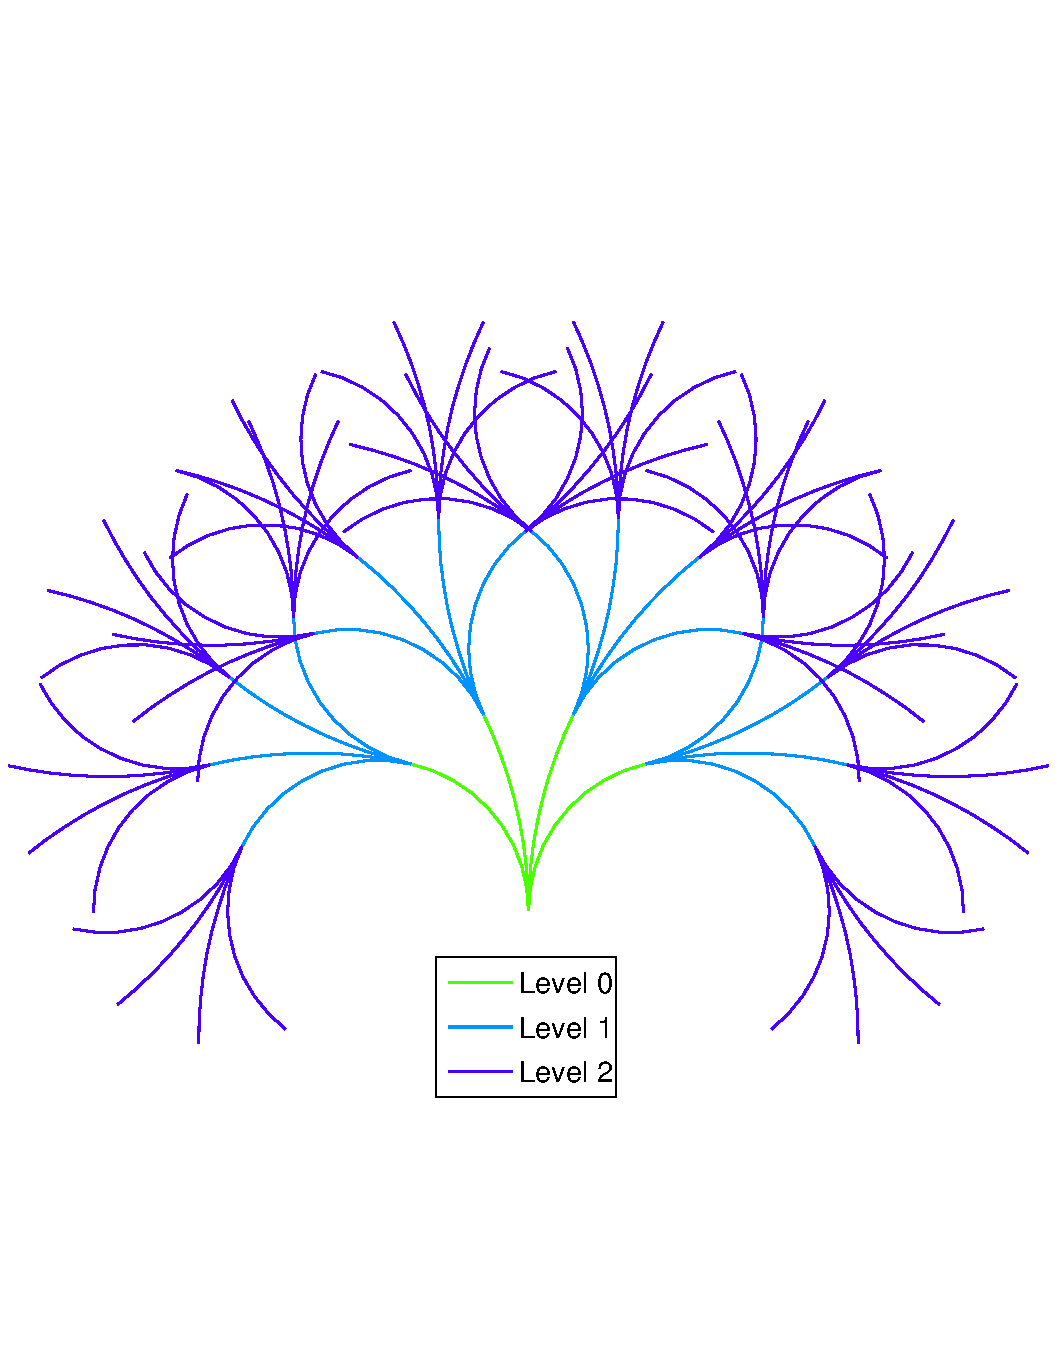
\includegraphics[width=0.7\textwidth, trim=10mm 45mm 10mm 80mm]{lattice_graph.pdf}
    \caption[A forward-arc motion primitive library.]{A primitive library with a depth of three constructed from a
    dictionary of four motion primitives. \label{fig:primitive_library}}
\end{figure}

A sampling of actions with varying $v$ and $w$ values (such as that depicted in
Fig.~\ref{fig:motion_prims}) is referred to as a
primitive \textit{dictionary}. To generate more actions, one can construct a
primitive \textit{library}. This is accomplished by forming a tree with nodes
corresponding to poses at the endpoints of actions. The tree is initialized by adding
the robot's current position as the root node. Then, a dictionary of motion
primitives is rotated and translated to leaf nodes in the tree until a specified
depth is reached. A primitive library is shown in
Fig.~\ref{fig:primitive_library}.
%
%\begin{figure}
%  \centering
%  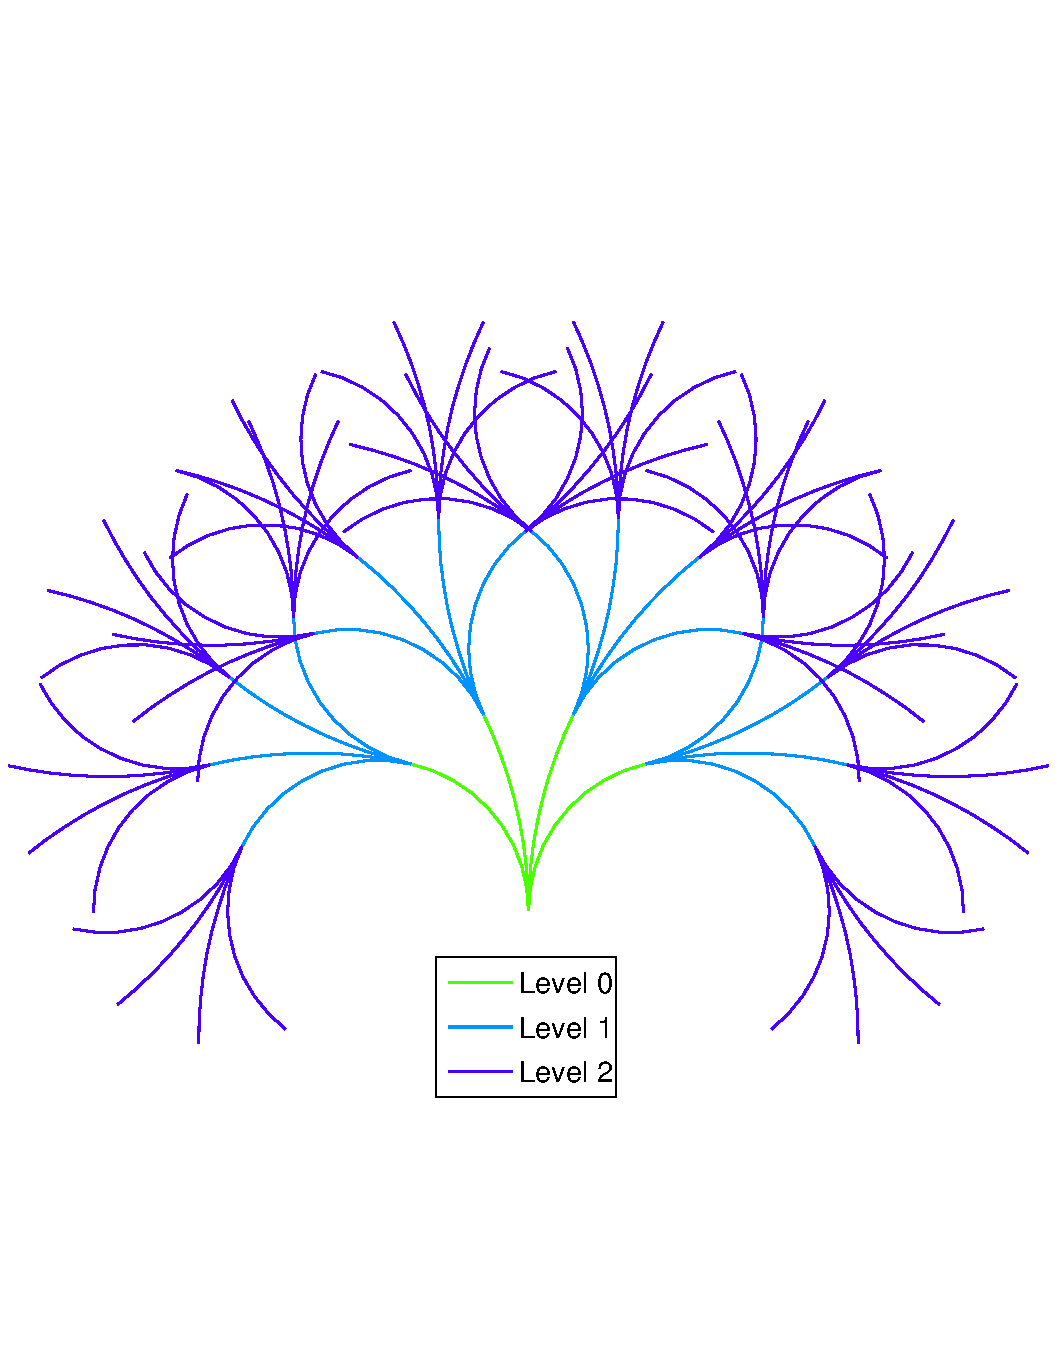
\includegraphics[width=0.7\textwidth, trim=10mm 45mm 10mm 80mm]{lattice_graph.pdf}
%  \caption[A forward-arc motion primitive library.]{A primitive library with a depth of three constructed from a
%  dictionary of four motion primitives. \label{fig:primitive_library}}
%\end{figure}

Forward-arc motion primitives are pre-computed prior to deployment into an
unknown environment, making them an efficient choice for real-time exploration. Collision
checking involves stepping along actions during a breadth-first or depth-first search and
pruning all nodes (actions) that lie below those that contain a collision.

\subsection{Lattice Graph Motion Primitives}
\label{subsec:lg_motion_primitives}

A third method for generating actions is lattice graph planning. Lattice graph
planners define a discrete set of goal states, and
solve Boundary Value Problems (BVPs) to find trajectories from $(\emptyset)$ to
each goal~\cite{pivtoraiko2005generating,pivtoraiko2009differentially,pivtoraiko2013incremental}
(Fig.~\ref{fig:lattice_graph}). The resulting set of motion primitives can
be rotated and translated to the robot's current position at run-time, and sampled
from to produce candidate actions. Like forward-arc motion primitives, lattice
graph motion primitives can be pre-computed and are therefore a suitable choice for
real-time exploration. Collision checking for motion primitives in the lattice
graph involves stepping along the action and checking for poses that lie outside
of the robot's configuration space.
%
\begin{figure}[h]
  \centering
  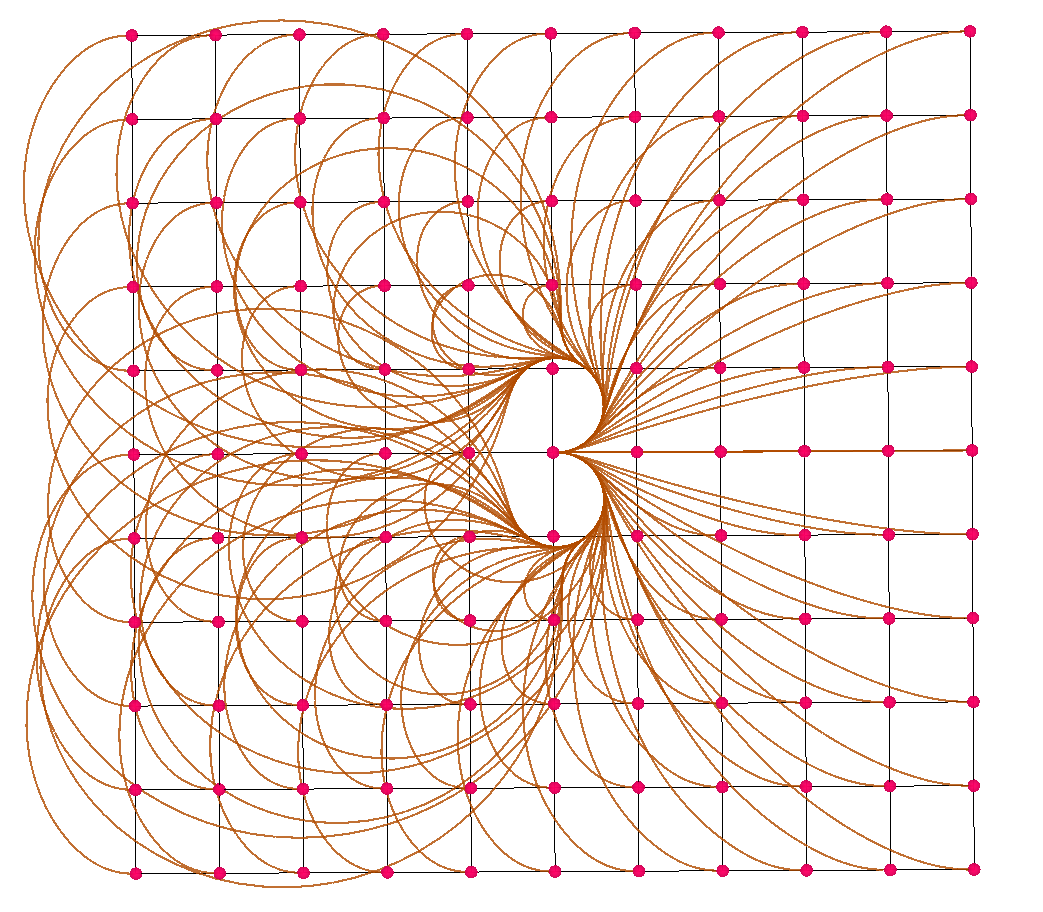
\includegraphics[width=0.45\textwidth]{lattice_graph_white.png}
  \caption[A lattice graph of motion primitives.]{An $11\times 11 \times 1$ lattice graph generated by solving many
    BVPs
  from the robot's initial pose (middle, facing right) to a lattice of final
poses (with final angle equal to initial angle) subject to linear and angular velocity
constraints. \label{fig:lattice_graph}}
\end{figure}

\section{Generalized Entropies and Divergences}
\label{sec:entropy_and_divergence}

Two fundamental building blocks of information theory that will be used to
formulate occupancy grid compression in Chapters~\ref{chapter3}
and~\ref{chapter4} are entropy and
divergence. The former describes the amount of uncertainty in a random variable,
or equivalently, the random variable's information content. The latter is a
distance metric between probability distributions that describes the
information lost when one distribution is used to describe another.
The most well-known forms of entropy and divergence are the Shannon
entropy~\cite{shannon1948mathematical}, and
Kullback-Leibler divergence~\cite{kullback1951information}. For a random variable
$X$, the Shannon entropy, $\text{H}$, and Kullback-Leibler divergence,
$\text{D}_{\text{KL}}$, are given by
%
\eq{
  \text{H}\left(X\right)
  &=
  - \sum_{x \in \mc{X}} p(x) \log_{2} p(x),
  \\[1cm]
  \text{D}_{\text{KL}}
  \left(p \vert \vert q\right)
  &=
  \sum_{x \in \mc{X}}
  p(x)
  \log_{2}
  \frac
  {p(x)}
  {q(x)},
}
%
where $\mc{X}$ is the sample space of $X$, and $p$ and $q$ are discrete probability
distributions over $X$. While Shannon entropy and Kullback-Leibler divergence
succinctly describe critical concepts of information theory, alternative definitions of
these concepts exist.

Shannon entropy is one solution to a more general parametric family of
entropies introduced by R\'{e}nyi~\cite{renyi1961measures} that take the
form
%
\eq{
  \text{H}_{\alpha}\left(X\right)
  &=
  \frac{1}{1-\alpha}
  \log_{2}
  \sum_{x \in \mc{X}}
  p^{\alpha}\left(x\right)
  \quad \text{(discrete)}
  \\[1cm]
  \text{H}_{\alpha}\left(X\right)
  &=
  \frac{1}{1-\alpha}
  \log_{2}
  \int_{\mc{X}}
  p^{\alpha}\left(x\right)
  \quad \text{(continuous)}.
}
%
R\'{e}nyi's so-called \textit{$\alpha$-entropy} approaches the Shannon entropy as $\alpha
\rightarrow 1$, but allows one to express the information content of a
random variable using any choice from a family of functions. $\text{H}_{\infty}$
entropy or $\text{H}_{2}$ entropy, for example, carry a similar meaning to
Shannon entropy, but in some cases may be easier to evaluate.
R\'{e}nyi's $\alpha$-entropy will be
used for an optimization that is difficult to solve using Shannon's entropy in
Chapter~\ref{chapter3}.

In a similar nature, there exists a spectrum of divergence measures that
generalize and extend the properties of the Kullback-Leibler divergence. The
Cauchy-Schwarz (CS) divergence is one measure that is of
particular importance to this thesis. Cauchy-Schwarz divergence can be derived by
substituting two
distributions, $p$ and $q$ into the Cauchy-Schwarz inequality~\cite{rudin1964principles}:
%
\eq{
  \sqrt{
    \sum_{x \in \mc{X}}
    p^{2}(x)
    \sum_{x \in \mc{X}}
    q^{2}(x)
  }
  &\ge
  \sum_{x \in \mc{X}}
  p(x)
  q(x)
  \quad \text{(discrete)}
  %\\[1cm]
  \\
  \sqrt{
    \int_{\mc{X}}
    p^{2}(x)dx
    \int_{\mc{X}}
    q^{2}(x)dx
  }
  &\ge
  \int_{\mc{X}}
  p(x)
  q(x)
  dx
  \quad \text{(continuous)}.
  \label{eq:cs_inequality}
}

Cauchy-Schwarz divergence measures the extent of this inequality.
%
\eq{
  \text{D}_{\text{CS}}
  \left(p \vert \vert q\right)
  &=
  \log
  \frac
  {
    \sum\limits_{x \in \mc{X}}
    p^{2}(x)
    \sum\limits_{x \in \mc{X}}
    q^{2}(x)
  }
  {
    \left(
    \sum\limits_{x \in \mc{X}}
    p(x)
    q(x)
    \right)^{2}
  }
  \quad \text{(discrete)}
  \\[1cm]
  \text{D}_{\text{CS}}
  \left(p \vert \vert q\right)
  &=
  \log
  \frac
  {
    \int_{\mc{X}}
    p^{2}(x) dx
    \int_{\mc{X}}
    q^{2}(x) dx
  }
  {
    \left(
    \int_{\mc{X}}
    p(x)
    q(x)
    dx
    \right)^{2}
  }
  \quad \text{(continuous)}.
  \label{eq:cs_divergence}
}
%
Cauchy-Schwarz divergence is a non-negative distance metric that takes on a value of zero
when its arguments are the same distribution. Unlike Kullback-Leibler
divergence, Cauchy-Schwarz divergence is symmetric in its arguments. It can equivalently be written in
terms of R\'{e}nyi's $\alpha$-entropy for $\alpha=2$.
%
\eq
{
  \text{D}_{\text{CS}}
  \left(p(x) \vert \vert q(y)\right)
  &=
  -2\log
  \int_{\mc{X}, \mc{Y}}
  p(x) q(y)
  dx dy
  +
  \log
  \int_{\mc{X}}
  p^{2}(x)
  dx
  +
  \log
  \int_{\mc{Y}}
  q^{2}(y)
  dy \\
  &=
  2 \text{H}_{2}\left(X; Y\right)
  - \text{H}_{2}\left(X\right)
  - \text{H}_{2}\left(Y\right),
  \label{eq:csd_entropy_decomp}
}
%
where $\text{H}_{2}\left(X; Y\right)$ is the quadratic R\'{e}nyi
cross-entropy~\cite{rao2008learning}:
%
\eq
{
  \text{H}_{2}\left(X;Y\right)
  &=
  -\log_{2}
  \sum_{x \in \mc{X}, y \in \mc{Y}}
  p(x)q(y)
  \quad \text{(discrete)}
  \\[1cm]
  \text{H}_{2}\left(X;Y\right)
  &=
  -\log_{2}
  \int
  p(x)
  q(y)
  dx dy
  \quad \text{(continuous)}.
  \label{eq:cross_entropy}
}

\section{Cauchy-Schwarz Quadratic Mutual Information}
\label{sec:csqmi}

The Cauchy-Schwarz divergence metric described in Section~\ref{sec:entropy_and_divergence} can be
used to define a second distance metric that measures the amount of dependence
between two random variables $X$ and $Y$. The amount of dependence between two
random variables is synonymous with the definition of mutual information, another
fundamental building block of information theory. Mutual information metrics
describe the difference between a joint distribution, $p(x, y)$, and the product
of its marginals, $p(x)p(y)$. Like entropy and divergence, there exists a common
definition for mutual information (the \textit{Shannon mutual information} (SMI)) that can be
extended and generalized. In the context of mobile robotic exploration, a more convenient
definition of mutual information is the \textit{Cauchy-Schwarz Quadratic mutual
information} (CSQMI), which is derived
by substituting $p(x, y)$ for $p$ and $p(x)p(y)$ for $q$
in~\eqref{eq:cs_divergence}.
%
\eq{
  \text{I}_{\text{CS}}
  \left(
    X;
    Y
  \right)
  &=
  \log
  \frac
  {
    \int_{\mc{X}}
    \int_{\mc{Y}}
    p^{2}(x,y) dx dy
    \int_{\mc{X}}
    \int_{\mc{Y}}
    p^{2}(x)p^{2}(y) dx dy
  }
  {
    \left(
    \int_{\mc{X}}
    \int_{\mc{Y}}
    p(x,y)
    p(x)p(y)
    dx dy
    \right)^{2}
  }.
  \label{eq:csqmi}
}
%
Charrow et al. originally showed that the CSQMI between a robot's map and a beam-based
sensor measurement is a superior reward metric to SMI for
exploration~\cite{charrow2015icra}. This is because CSQMI can be computed
analytically without requiring an expensive sampling step to
calculate the expected value of a future sensor measurement. Additionally,
CSQMI can be computed exactly in $\mc{O}(n^2)$, and to a close approximation
in $\mc{O}(n)$, where $n$ is the number of cells in the robot's map intersected by a
sequence of beam-based sensor measurements $\mbf{z}_{\mbf{\tau}}$. While SMI can also be approximated in time linear in
$n$, Charrow et al. show that CSQMI has a smaller linear constant factor,
allowing CSQMI to be computed in roughly one seventh of the amount of time.
Like SMI, CSQMI is non-negative and zero only when its arguments are independent
(i.e. when $p(x, y) = p(x)p(y)$). Figure~\ref{fig:mi_vs_csqmi} shows that CSQMI and SMI are
similar when evaluated on an OG with a beam-based sensor model, and control actions
that maximize CSQMI guide the robot to unexplored space. The reader should refer
to Charrow et al.~\cite{charrow2015icra} for discussion regarding
explicit calculation of CSQMI between an OG map and a beam-based sensor
measurement.

Given the numerous benefits of CSQMI, $\text{I}_{\text{CS}}\left(\mbf{m};\mbf{z}_{\mbf{\tau}}\left(\mbf{x}_{\mbf{\tau}}\right)\right)$
is a suitable choice
for $\mc{J}\left(\mbf{m}; \mbf{z}_{\mbf{\tau}}\left(\mbf{x}_{\mbf{\tau}}\right)\right)$
in~\eqref{eq:active_perception}. The CSQMI between an OG map and sequence of
beam-based measurements is
%
\eq{
  \text{I}_{\text{CS}}
  \left(
  \mbf{m}; \mbf{z}_{\mbf{\tau}}
  \right)
  &=
  \log
  \frac
  {
    \int
    \sum_{\mc{M}}
    p^{2}(\mbf{m}, \mbf{z}_{\mbf{\tau}})
    d\mbf{z}_{\mbf{\tau}}
    \int
    \sum_{M}
    p^{2}(\mbf{m}) p^{2}(\mbf{z}_{\mbf{\tau}})
    d\mbf{z}_{\mbf{\tau}}
  }
  {
    \left(
    \int
    \sum_{\mc{M}}
    p(\mbf{m})p(\mbf{z}_{\mbf{\tau}})
    p(\mbf{m}, \mbf{z}_{\mbf{\tau}})
    d\mbf{z}_{\mbf{\tau}}
    \right)^{2}
  }.
}
%
The map $\mbf{m}$ has a discrete sample space $\mc{M}$ because cells may
only take on a value of $\texttt{OCC}$ or $\texttt{EMP}$. A map of $K$ cells
can therefore take on one of $\vert \mc{M} \vert = 2^{K}$ permutations.
Substituting $\text{I}_{\text{CS}}$ for $\mc{J}$ in~\eqref{eq:active_perception}
yields an active perception optimization that guides a robot towards unexplored
locations in its map by maximizing an information information-theoretic reward functional.
%
\eq
{
 \mbf{x}_{\mbf{\tau}}^{*}
 &=
 \argmax_{\mbf{x}_{\mbf{\tau}} \in \hat{\mc{X}}}
 \
 \text{I}_{\text{CS}}\left(\mbf{m},
 \mbf{z}_{\mbf{\tau}}(\mbf{x}_{\mbf{\tau}})\right).
 \label{eq:active_perception_csqmi}
}

\section{Summary of Foundations}

Chapter~\ref{chapter2} reviewed foundational elements that will be used for
derivations in the remaining chapters. These elements culminate in an
optimization that drives a robot towards unexplored space in its map by
maximizing an information-theoretic reward
function~\eqref{eq:active_perception_csqmi}. The chosen reward function,
CSQMI~\cite{principe2010information},
resembles Shannon's original definition of mutual information, but can be computed
more efficiently when its arguments are an OG map and a sequence
of beam-based sensor measurements~\cite{charrow2015icra}.

Furthermore, Chapter~\ref{chapter2} discussed three methods for generating
dynamically feasible and collision-free actions through the robot's
configuration space. The action maximizing CSQMI (either integrated over the
path, or at the action's final pose) will be chosen as that which optimally
drives the robot towards unexplored space. The remainder of this thesis will use both forward-arc
motion primitives and lattice graph motion primitives for action generation,
although the third option - frontier seeding - is equally viable.

%

% ====================================================================
%    Chapter 3
% ====================================================================
%
\chapter{Test 1 - Chapter}
\section{Test 1 - Section}

%

% ====================================================================
%    Chapter 4
% ====================================================================
%
%\chapter{Balancing Map Compression with Sensing Accuracy}
\chapter{}
\label{chapter4}

The PRI strategy in Sec.~\ref{subsec:pri} determines an optimal compression given a desired OG resolution. However, Fig.~\ref{fig:csqmi_timing} suggests that one should also reduce the resolution of the OG as much as possible to increase efficiency. In this section we formulate a second optimization based on the Information Bottleneck (IB) method~\cite{tishby2000information} that chooses a grid resolution minimizing both the redundancy between $m^{K}$ and
$C_{n}(m^{K})$, and loss of mutual information with respect to a sensor measurement $z$.


\section{The Information Bottleneck Method}

IB is a widely used technique in signal processing for finding the optimal reduced representation $\hat{X}$ of a random variable $X$ that preserves maximum information about a second random variable $Y$:
%
\eq{
    \min_{\hat{X}}
    \text{I}(X; \hat{X})
    -
    \beta
    \text{I}(\hat{X}; Y).
    \label{eq:ib_opt}
}

IB resembles PRI, but considers the effects of compression on the information between two datasets, as opposed to one. Similar to $\lambda$ in the PRI optimization, $\beta$ is a design parameter that trades compression for conservation of information. As $\beta \rightarrow 0$, the optimization tends towards the trivial lossy compression $\{\hat{X}\}=0$, whereas when $\beta \rightarrow \infty$, $\hat{X}$ approaches its original representation $X$~\cite{principe2010information}. The two terms in the argument of~\eqref{eq:ib_opt} can equivalently be thought of as the information loss incurred by describing $\hat{X}$ with $Y$ instead of with $X$~\cite{geiger2011information}.

Most importantly for OG compression, when combined with the PRI approach in Section~\ref{subsec:pri}, the IB method can be used to find an optimal compression $n^{*}$:
%
\begin{gather}
    n^{*}
    =
    \argmin_{
        n \in \mbb{N}_{0}
    } \, \,
    \text{I}_{\text{CS}}\left(m^{K}; C_{n}(m^{K})\right)
    -
    \beta
    \text{I}_{\text{CS}}\left(C_{n}(m^{K}); z\right).
    \label{eq:ib_arg_opt}
\end{gather}

\section{Optimizing Map Resolution for Sensing}

The second term can be computed using~\eqref{eq:csqmi}, and is $2^{1\times n}$ times more efficient than computing~\eqref{eq:csqmi} with respect to the uncompressed map $m^{K}$ (where $d=1$ because $\text{I}_{\text{CS}}(m;z_{\tau})$ is computed using 1D raycasts). Since $\text{I}_{\text{CS}}(m^{K};C_{n}(m^{K}))$ describes the divergence between the distributions $p(m^{K},C_{n}(m^{K}))$ and $p(m^{K})p(C_{n}({m}^{K}))$, the first term in~\eqref{eq:csqmi} can be computed by substituting these for $p(x_i)$ and $p(\hat{x}_{i})$ in the definition of Cauchy-Schwarz divergence~\eqref{eq:cs_divergence}.

However, the joint distribution $p(m^{K},C_{n}(m^{K}))$ is underdetermined by two variables, and must be constrained before computing~\eqref{eq:ib_arg_opt}. While the remaining two degrees of freedom make the IB cost function arbitrary for a single resolution, fixing the joint distribution and using it to compute CSQMI across different grid resolutions still yields a meaningful optimization. To constrain the extra degrees of freedom we first decompose the joint distribution into independent regions $r \in m^{K}$:
%
\eq{
p(m^{K},C_{n}(m^{K}))
&=
\prod_{r \in m^{K}}
p(m^{R}_{r},C_{n}(m^{R}_{r})) \\
&=
\prod_{r \in m^{K}}
p(m^{R}_{r},\tilde{m}^{R}_{r}),
}

where the second equation holds by noting $C_{n}(m^{R}_{r})$ has a dimension of one, and that that all cells in $\tilde{m}^{r}$ are completely determined by knowing $C_{n}(m^{R}_{r})$. Then, for each region $r$, we choose the joint distribution $p(m^{R}_{r},\tilde{m}^{R}_{r}))$ to be a product of the marginals $p(m^{R}_{r})$ and $p(\tilde{m}^R_{r}))$, weighted by four extra coefficients $w_{1:4}$ (Table~\ref{tab:contingency}). Similar to the reasons that $\eta$ in Sec.~\ref{subsec:pri} is chosen to preserve occupied cells through compression, the constant $c_1 \in (0, 1)$ downweighs the probability of the event that $\tilde{m}^{R}$ is $\{\texttt{EMP},\dots,\texttt{EMP}\}$ if any grid cells in $m^{R}$ are occupied. The remaining three constants balance the effects of $w_{1}$ such that the conditional distributions over the rows and columns of Table~\ref{tab:contingency} all sum to the marginal distributions on the bottom-most row and right-most column.

%the first term can be computed by substituting $p(m^{K},C_{n}(m^{K}))$ and $p(m^{K})p(C_{n}({m}^{K}))$ for $p(x_i)$ and $p(\hat{x}_{i})$ in~\eqref{eq:cs_divergence}, respectively. However, the joint distribution $p(m^{K},C_{n}(m^{K}))$

%derivation in Sec.~\ref{subsec:pri} left the joint distribution $p(m^{R},\,\tilde{})$


%the first term cannot immediately be evaluated because the PRI compression derivation leaves the joint distribution $p(m^{R}, \tilde{m}^{R})$ underconstrained. While the remaining two degrees of freedom make the IB cost function arbitrary for a single resolution, fixing the joint and using it to compute CSQMI across different grid resolutions still yields a meaningful optimization. We choose the joint to be a product of the marginals $p(m^{R})$ and $p(\tilde{m}^{R})$, weighted by four extra coefficients $w_{1:4}$. Just as $\eta$ in Sec.~\ref{subsec:pri} is chosen to preserve occupied cells through compression, the constant $c_1 \in (0, 1)$ downweighs the probability of the event that $\tilde{m}^{R}$ is $\{\texttt{EMP},\dots,\texttt{EMP}\}$ if any grid cells in $m^{R}$ are occupied. The remaining three constants balance the effects of $w_{1}$ such that the conditional distributions in the rows and columns of Table~\ref{tab:contingency} all sum to the marginals. With the joint distribution fixed, the first term in~\eqref{eq:ib_arg_opt} can be computed by substituting $p(m^{R},\tilde{m}^{R})$ and $p(m^{R})p(\tilde{m}^{R})$ for $p(x_i)$ and $p(\hat{x}_{i})$ in~\eqref{eq:cs_divergence}, respectively.

Figure~\ref{fig:loss_compression} displays the influence of $\beta$ on the IB optimization for a multi-beam measurement captured from a planned future location. The optimization favors no compression when $\beta$ is large, and maximum compression when $\beta$ is small.

\begin{figure}
    \centering
    \begin{subfigure}[t]{0.45\textwidth}
        \centering
        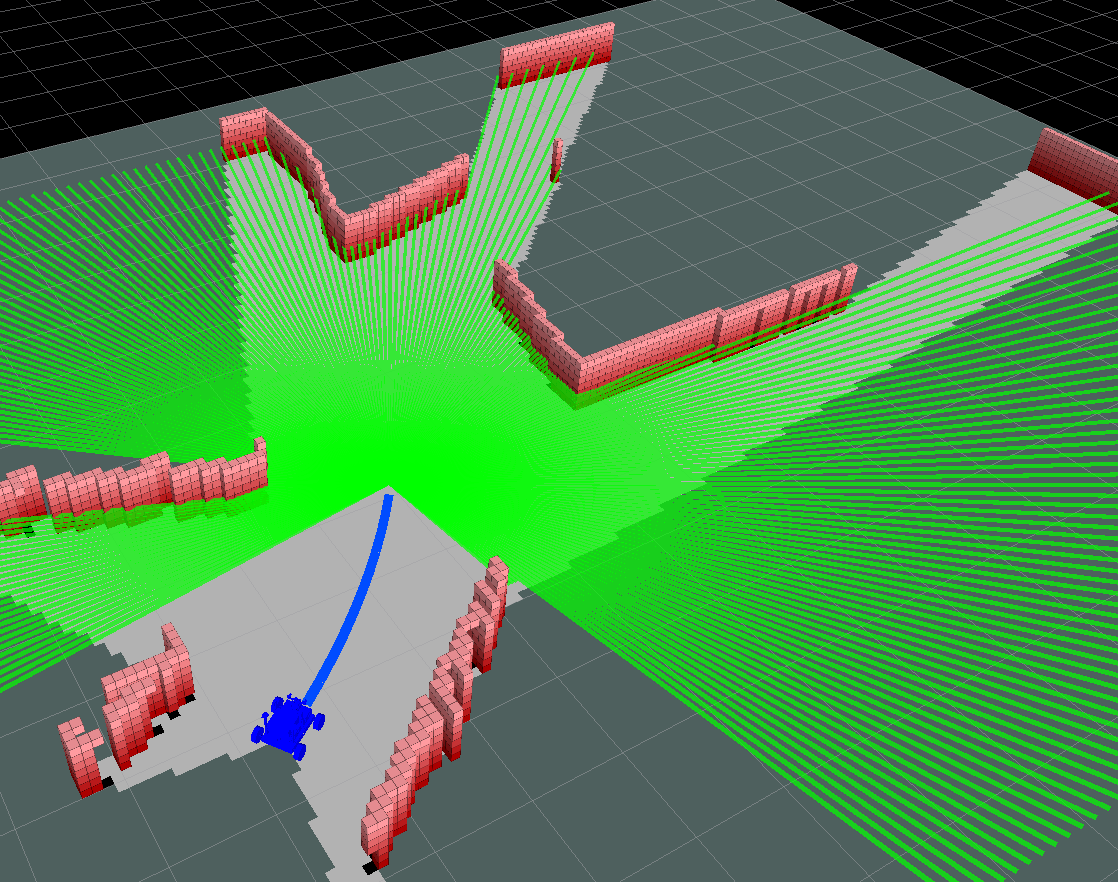
\includegraphics[height=5.2cm]{plan_ahead.png}
        \caption{\label{fig:loss_compression1}}
    \end{subfigure}
    \hfill
    \begin{subfigure}[t]{0.45\textwidth}
        \centering
        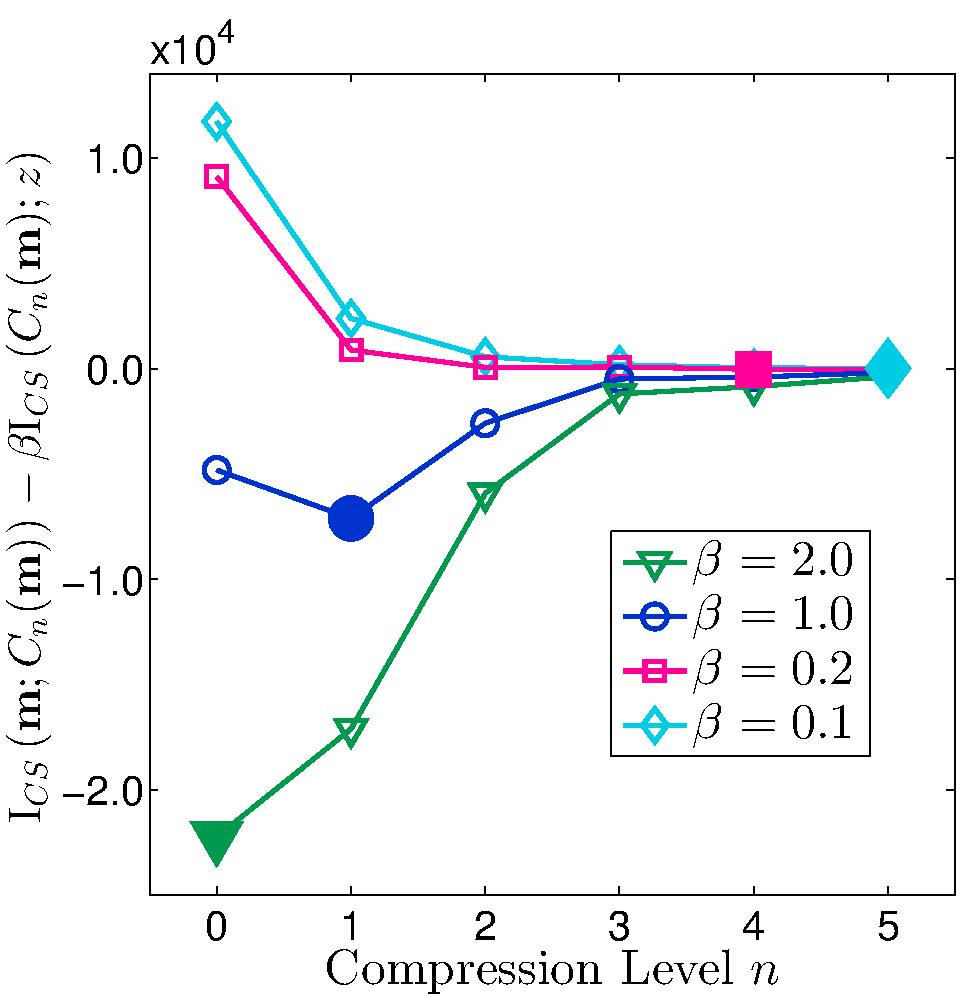
\includegraphics[height=5.2cm]{beta.pdf}
        \caption{\label{fig:loss_compression2}}
    \end{subfigure}
    \caption{\ref{fig:loss_compression1} shows an uncompressed map and measurement taken from a planned future position. With this map and expected laser scan, the optimal compression level (filled markers) computed with~\eqref{eq:ib_arg_opt} decreases as $\beta$ increases, favoring preservation of information about the measurement as opposed to compression (\ref{fig:loss_compression2}). \label{fig:loss_compression}}
\end{figure}

\section{Results}

\section{Chapter Summary}

%

% ====================================================================
%    Chapter 5
% ====================================================================
%
\chapter{Test 5 - Chapter}

%

% ====================================================================
%    References
% ====================================================================
%
\addcontentsline{toc}{chapter}{Bibliography}
\bibliography{content/refs}

\end{document}
